% Options for packages loaded elsewhere
\PassOptionsToPackage{unicode}{hyperref}
\PassOptionsToPackage{hyphens}{url}
\PassOptionsToPackage{dvipsnames,svgnames,x11names}{xcolor}
%
\documentclass[
  letterpaper,
]{scrreprt}\usepackage{amsmath,amssymb}
\usepackage{lmodern}
\usepackage{iftex}
\ifPDFTeX
  \usepackage[T1]{fontenc}
  \usepackage[utf8]{inputenc}
  \usepackage{textcomp} % provide euro and other symbols
\else % if luatex or xetex
  \usepackage{unicode-math}
  \defaultfontfeatures{Scale=MatchLowercase}
  \defaultfontfeatures[\rmfamily]{Ligatures=TeX,Scale=1}
\fi
% Use upquote if available, for straight quotes in verbatim environments
\IfFileExists{upquote.sty}{\usepackage{upquote}}{}
\IfFileExists{microtype.sty}{% use microtype if available
  \usepackage[]{microtype}
  \UseMicrotypeSet[protrusion]{basicmath} % disable protrusion for tt fonts
}{}
\makeatletter
\@ifundefined{KOMAClassName}{% if non-KOMA class
  \IfFileExists{parskip.sty}{%
    \usepackage{parskip}
  }{% else
    \setlength{\parindent}{0pt}
    \setlength{\parskip}{6pt plus 2pt minus 1pt}}
}{% if KOMA class
  \KOMAoptions{parskip=half}}
\makeatother
\usepackage{xcolor}
\IfFileExists{xurl.sty}{\usepackage{xurl}}{} % add URL line breaks if available
\IfFileExists{bookmark.sty}{\usepackage{bookmark}}{\usepackage{hyperref}}
\hypersetup{
  pdftitle={Climate Change in Montana},
  pdfauthor={Colin Brust},
  colorlinks=true,
  linkcolor={blue},
  filecolor={Maroon},
  citecolor={Blue},
  urlcolor={Blue},
  pdfcreator={LaTeX via pandoc}}
\urlstyle{same} % disable monospaced font for URLs
\setlength{\emergencystretch}{3em} % prevent overfull lines
\setcounter{secnumdepth}{5}
% Make \paragraph and \subparagraph free-standing
\ifx\paragraph\undefined\else
  \let\oldparagraph\paragraph
  \renewcommand{\paragraph}[1]{\oldparagraph{#1}\mbox{}}
\fi
\ifx\subparagraph\undefined\else
  \let\oldsubparagraph\subparagraph
  \renewcommand{\subparagraph}[1]{\oldsubparagraph{#1}\mbox{}}
\fi


\providecommand{\tightlist}{%
  \setlength{\itemsep}{0pt}\setlength{\parskip}{0pt}}\usepackage{longtable,booktabs,array}
\usepackage{calc} % for calculating minipage widths
% Correct order of tables after \paragraph or \subparagraph
\usepackage{etoolbox}
\makeatletter
\patchcmd\longtable{\par}{\if@noskipsec\mbox{}\fi\par}{}{}
\makeatother
% Allow footnotes in longtable head/foot
\IfFileExists{footnotehyper.sty}{\usepackage{footnotehyper}}{\usepackage{footnote}}
\makesavenoteenv{longtable}
\usepackage{graphicx}
\makeatletter
\def\maxwidth{\ifdim\Gin@nat@width>\linewidth\linewidth\else\Gin@nat@width\fi}
\def\maxheight{\ifdim\Gin@nat@height>\textheight\textheight\else\Gin@nat@height\fi}
\makeatother
% Scale images if necessary, so that they will not overflow the page
% margins by default, and it is still possible to overwrite the defaults
% using explicit options in \includegraphics[width, height, ...]{}
\setkeys{Gin}{width=\maxwidth,height=\maxheight,keepaspectratio}
% Set default figure placement to htbp
\makeatletter
\def\fps@figure{htbp}
\makeatother
\newlength{\cslhangindent}
\setlength{\cslhangindent}{1.5em}
\newlength{\csllabelwidth}
\setlength{\csllabelwidth}{3em}
\newlength{\cslentryspacingunit} % times entry-spacing
\setlength{\cslentryspacingunit}{\parskip}
\newenvironment{CSLReferences}[2] % #1 hanging-ident, #2 entry spacing
 {% don't indent paragraphs
  \setlength{\parindent}{0pt}
  % turn on hanging indent if param 1 is 1
  \ifodd #1
  \let\oldpar\par
  \def\par{\hangindent=\cslhangindent\oldpar}
  \fi
  % set entry spacing
  \setlength{\parskip}{#2\cslentryspacingunit}
 }%
 {}
\usepackage{calc}
\newcommand{\CSLBlock}[1]{#1\hfill\break}
\newcommand{\CSLLeftMargin}[1]{\parbox[t]{\csllabelwidth}{#1}}
\newcommand{\CSLRightInline}[1]{\parbox[t]{\linewidth - \csllabelwidth}{#1}\break}
\newcommand{\CSLIndent}[1]{\hspace{\cslhangindent}#1}

\makeatletter
\@ifpackageloaded{tcolorbox}{}{\usepackage[many]{tcolorbox}}
\@ifpackageloaded{fontawesome5}{}{\usepackage{fontawesome5}}
\definecolor{quarto-callout-color}{HTML}{909090}
\definecolor{quarto-callout-note-color}{HTML}{0758E5}
\definecolor{quarto-callout-important-color}{HTML}{CC1914}
\definecolor{quarto-callout-warning-color}{HTML}{EB9113}
\definecolor{quarto-callout-tip-color}{HTML}{00A047}
\definecolor{quarto-callout-caution-color}{HTML}{FC5300}
\definecolor{quarto-callout-color-frame}{HTML}{acacac}
\definecolor{quarto-callout-note-color-frame}{HTML}{4582ec}
\definecolor{quarto-callout-important-color-frame}{HTML}{d9534f}
\definecolor{quarto-callout-warning-color-frame}{HTML}{f0ad4e}
\definecolor{quarto-callout-tip-color-frame}{HTML}{02b875}
\definecolor{quarto-callout-caution-color-frame}{HTML}{fd7e14}
\makeatother
\makeatletter
\makeatother
\makeatletter
\@ifpackageloaded{caption}{}{\usepackage{caption}}
\AtBeginDocument{%
\ifdefined\contentsname
  \renewcommand*\contentsname{Table of contents}
\else
  \newcommand\contentsname{Table of contents}
\fi
\ifdefined\listfigurename
  \renewcommand*\listfigurename{List of Figures}
\else
  \newcommand\listfigurename{List of Figures}
\fi
\ifdefined\listtablename
  \renewcommand*\listtablename{List of Tables}
\else
  \newcommand\listtablename{List of Tables}
\fi
\ifdefined\figurename
  \renewcommand*\figurename{Figure}
\else
  \newcommand\figurename{Figure}
\fi
\ifdefined\tablename
  \renewcommand*\tablename{Table}
\else
  \newcommand\tablename{Table}
\fi
}
\@ifpackageloaded{float}{}{\usepackage{float}}
\floatstyle{ruled}
\@ifundefined{c@chapter}{\newfloat{codelisting}{h}{lop}}{\newfloat{codelisting}{h}{lop}[chapter]}
\floatname{codelisting}{Listing}
\newcommand*\listoflistings{\listof{codelisting}{List of Listings}}
\makeatother
\makeatletter
\@ifpackageloaded{caption}{}{\usepackage{caption}}
\@ifpackageloaded{subcaption}{}{\usepackage{subcaption}}
\makeatother
\makeatletter
\@ifpackageloaded{tcolorbox}{}{\usepackage[many]{tcolorbox}}
\makeatother
\makeatletter
\@ifundefined{shadecolor}{\definecolor{shadecolor}{rgb}{.97, .97, .97}}
\makeatother
\makeatletter
\makeatother
\ifLuaTeX
  \usepackage{selnolig}  % disable illegal ligatures
\fi

\title{Climate Change in Montana}
\author{Colin Brust}
\date{11/2/2022}

\begin{document}
\maketitle

\ifdefined\Shaded\renewenvironment{Shaded}{\begin{tcolorbox}[interior hidden, borderline west={3pt}{0pt}{shadecolor}, breakable, boxrule=0pt, frame hidden, enhanced, sharp corners]}{\end{tcolorbox}}\fi

\renewcommand*\contentsname{Table of contents}
{
\hypersetup{linkcolor=}
\setcounter{tocdepth}{2}
\tableofcontents
}
\hypertarget{overview}{%
\chapter*{Overview}\label{overview}}
\addcontentsline{toc}{chapter}{Overview}

Understanding current climate change and projecting future climate
trends are of vital importance--both for our economy and our well-being.
It is our goal to provide science-based information that serves as a
resource for \emph{Montanans} who are interested in understanding
\emph{Montana}'s climate and its impacts on water, agricultural lands
and forests. To provide this understanding, we can learn from past
climate trends. However, knowledge of the past is only partially
sufficient in preparing for a future defined by unprecedented levels of
greenhouse gases in the atmosphere. Therefore, we also provide
projections of change into the future using today's best scientific
information and modeling techniques.

\hypertarget{key-messages}{%
\section*{Key Messages}\label{key-messages}}
\addcontentsline{toc}{section}{Key Messages}

Annual average temperatures, including daily minimums, maximums, and
averages, have risen across the state between 1950 and 2015. The
increases range between \textbf{2.0-3.0°F (1.1-1.7°C)} during this
period.

Winter and spring in Montana have experienced the most warming. Average
temperatures during these seasons have risen by \textbf{3.9°F (2.2°C)}
between 1950 and 2015.

Montana's growing season length is increasing due to the earlier onset
of spring and more extended summers; we are also experiencing more warm
days and fewer cool nights. From \textbf{1951-2010}, the growing season
increased by \textbf{12} days. In addition, the annual number of warm
days has increased by \textbf{2.0\%} and the annual number of cool
nights has decreased by \textbf{4.6\%} over this period.

Despite no historical changes in average annual precipitation between
1950 and 2015, there have been changes in average seasonal precipitation
over the same period. Average winter precipitation has decreased by
\textbf{0.9 inches (2.3 cm)}, which can mostly be attributed to natural
variability and an increase in El Niño events, especially in the
\textbf{western and central parts of the state}. A significant increase
in spring precipitation \textbf{(1.3-2.0 inches {[}3.3-5.1 cm{]})} has
also occurred during this period for the \textbf{eastern portion} of the
state.

The state of Montana is projected to continue to warm in all geographic
locations, seasons, and under all emission scenarios throughout the 21st
century. By mid century, Montana temperatures are projected to increase
by approximately \textbf{4.5-6.0°F (2.5-3.3°C)} depending on the
emission scenario. By the end-of-century, Montana temperatures are
projected to increase \textbf{5.6-9.8°F (3.1-5.4°C)} depending on the
emission scenario. These state-level changes are larger than the average
changes projected globally and nationally.

The number of days in a year when daily temperature exceeds 90°F (32°C)
and the number of frost-free days are expected to increase across the
state and in both emission scenarios studied. Increases in the number of
days above 90°F (32°C) are expected to be greatest in the
\textbf{eastern} part of the state. Increases in the number of
frost-free days are expected to be greatest in the \textbf{western} part
of the state.

Across the state, precipitation is projected to increase in
\textbf{winter, spring, and fall;} precipitation is projected to
decrease in \emph{summer.} The largest increases are expected to occur
during \emph{spring} in the \emph{southern} part of the state. The
largest decreases are expected to occur during \emph{summer} in the
\emph{central} and \emph{southern} parts of the state.

\hypertarget{climate-change-defined}{%
\section*{Climate Change Defined}\label{climate-change-defined}}
\addcontentsline{toc}{section}{Climate Change Defined}

The US Global Change Research Program (USGCRP undated) defines climate
change as follows:

\begin{quote}
``Changes in average weather conditions that persist over multiple
decades or longer. Climate change encompasses both increases and
decreases in temperature, as well as shifts in precipitation, changing
risk of certain types of severe weather events, and changes to other
features of the climate system.''
\end{quote}

\hypertarget{outline}{%
\section*{Outline}\label{outline}}
\addcontentsline{toc}{section}{Outline}

This document focuses on three areas:

\begin{enumerate}
\def\labelenumi{\arabic{enumi}.}
\item
  providing a baseline summary of climate and climate change for
  Montana---with a focus on changes in temperature, precipitation, and
  extreme events---including reviewing the fundamentals of climate
  change science;
\item
  reviewing historical trends in Montana's climate, and what those
  trends reveal about how our climate has changed in the past century,
  changes that are potentially attributable to world-wide increases in
  greenhouse gases; and
\item
  considering what today's best available climate models project
  regarding Montana's future, and how certain we can be in those
  projections.
\end{enumerate}

This chapter serves as a foundation for the Montana Climate Assessment,
providing information on present-day climate and climate terminology,
past climate trends, and future climate projections. This foundation
then serves as the basis for analyzing three key sectors of
Montana---water, forests, and agriculture---considered in the other
chapters of this assessment. In the sections below, we introduce the
climate science and discuss important fundamental processes that
determine whether climate remains constant or changes.

\hypertarget{natural-and-human-causes-of-climate-change}{%
\chapter{Natural and Human Causes of Climate
Change}\label{natural-and-human-causes-of-climate-change}}

Climate is driven largely by radiation from the sun. Incoming solar
radiation may be reflected, absorbed by land surface and water bodies,
transformed (as in photosynthesis), or emitted from the land surface as
longwave radiation. Each of these processes influences climate through
changes to temperature, winds, the water cycle, and more. The overall
process is best understood by considering the Earth's energy budget.

\begin{tcolorbox}[standard jigsaw,colbacktitle=quarto-callout-note-color!10!white, bottomtitle=1mm, toptitle=1mm, rightrule=.15mm, leftrule=.75mm, titlerule=0mm, title={The Earth's Energy Budget}, arc=.35mm, bottomrule=.15mm, colframe=quarto-callout-note-color-frame, opacityback=0, opacitybacktitle=0.6, colback=white, left=2mm, toprule=.15mm, coltitle=black]
The Earth's climate is driven by the sun. The balance between incoming
and outgoing radiation---Earth's radiation or energy budget---determines
the energy available for changes in temperature, precipitation, and
winds and, hence, influences atmospheric chemistry and the hydrologic
cycle. The Earth's surface, atmosphere, and clouds absorb a portion of
incoming solar radiation, thereby increasing temperatures. Energy as
longwave radiation (heat) is re-emitted to the atmosphere, clouds, or
space, thereby reducing temperatures at the source. If the absorbed
solar radiation and emitted heat are in balance, the Earth's temperature
remains constant.

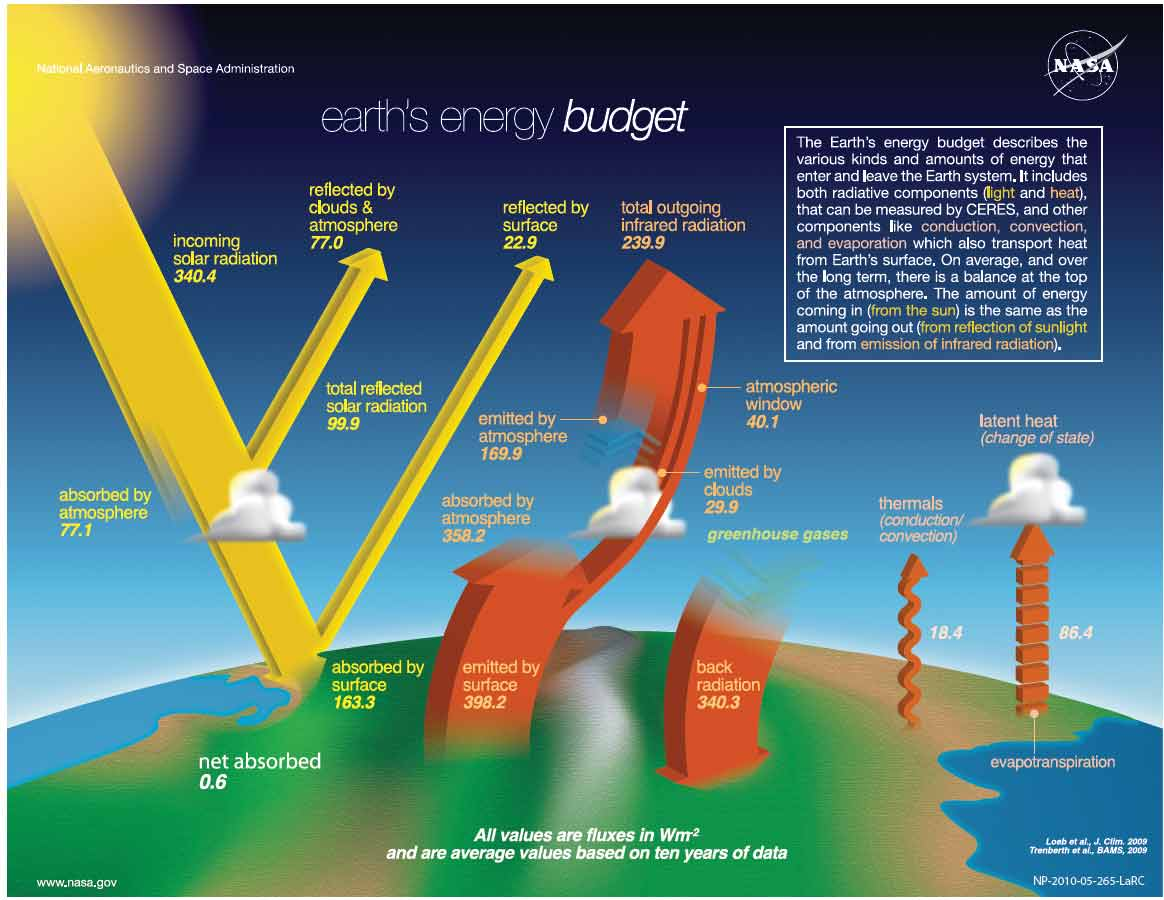
\includegraphics{./assets/energy-budget.jpg}
\end{tcolorbox}

Natural factors contributing to past climate change are well documented
and include changes in atmospheric chemistry, ocean circulation
patterns, solar radiation intensity, snow and ice cover, Earth's orbital
cycle around the sun, continental position, and volcanic eruptions.
While these natural factors are linked to past climate change, they are
also incorporated in the analysis of current climate change.

Since the Industrial Revolution, global climate has changed faster than
at any other time in Earth's history (Mann et al.~1999). This rapid rate
of change---often referred to as human-caused climate change---has
resulted from changes in atmospheric chemistry, specifically increases
in greenhouse gases due to increased combustion of fossil fuels,
land-use change (e.g., deforestation), and fertilizer production (Figure
2-1) (Forster et al.~2007). The primary greenhouse gases in the Earth's
atmosphere are carbon dioxide (CO2), methane (CH4), nitrous oxide (N2O),
water vapor (H2O), and ozone (O3).

\begin{figure}

{\centering 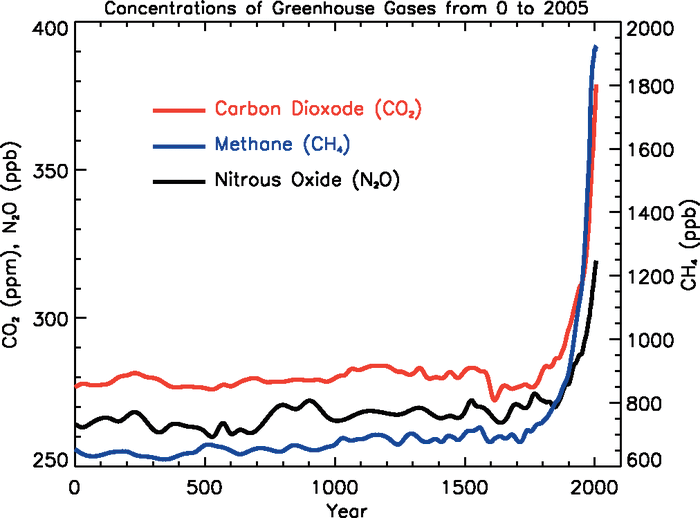
\includegraphics{./assets/ghg-emissions.png}

}

\caption{\label{fig-ghg}Changes in important global atmospheric
greenhouse gas concentrations from year 0 to 2005 AD (ppm, ppb = parts
per million and parts per billion, respectively) (Forster et al.~2007).}

\end{figure}

Incoming solar radiation is either absorbed, reflected, or re-radiated
from the Earth's surface. Since greenhouse gas concentrations are
greatest near the surface, a large fraction of this reflected and
re-radiated energy is absorbed in the lower portions of the atmosphere
(hence the increase in surface temperatures and the term ``greenhouse
effect''---see sidebar). For the total energy budget to balance, the
energy (and temperature) at the top of the atmosphere must decrease to
account for the increase of energy (and temperature) near the Earth's
surface.

At natural levels, greenhouse gases are crucial for life on Earth; they
help keep average global temperatures above freezing and at levels that
sustain plant and animal life. However, at the increased levels seen
since the Industrial Revolution (roughly 275 ppm then, 400 ppm now;
Figure~\ref{fig-ghg}), greenhouse gases are contributing to the rapid
rise of our global average temperatures by trapping more heat, often
referred to as human-caused climate change. In the following chapters,
we will refer to the impacts and effects of climate change as a result
of both natural variability and human-caused climate change.

\begin{tcolorbox}[standard jigsaw,colbacktitle=quarto-callout-note-color!10!white, bottomtitle=1mm, toptitle=1mm, rightrule=.15mm, leftrule=.75mm, titlerule=0mm, title={The Greenhouse Effect}, arc=.35mm, bottomrule=.15mm, colframe=quarto-callout-note-color-frame, opacityback=0, opacitybacktitle=0.6, colback=white, left=2mm, toprule=.15mm, coltitle=black]
The Earth's climate is driven by the sun. The high temperature of the
sun results in the emission of high energy, shortwave radiation. About
31\% of the shortwave radiation from the sun is reflected back to space
by clouds, air molecules, dust, and lighter colored surfaces on the
earth. Another 20\% of the shortwave radiation is absorbed by ozone in
the upper atmosphere and by clouds and water vapor in the lower
atmosphere. The remaining 49\% is transmitted through the atmosphere to
the land surfaces and oceans and is absorbed. The Earth's surface
re-emits about 79\% of the absorbed energy as longwave radiation. Unlike
shortwave radiation, the Earth's atmosphere absorbs approximately 90\%
of the longwave radiation emitted from objects on its surface. This
results because of the presence of gases such as water vapor, carbon
dioxide (CO2), methane (CH4), nitrous oxide (N2O), and various
industrial products (e.g.~chlorofluorocarbons; CFCs) that more
effectively absorb longwave radiation. In turn, the energy absorbed by
these gases is reradiated in all directions. The portion that is
redirected back towards the surface contributes to warming and a
phenomenon known as the greenhouse effect.

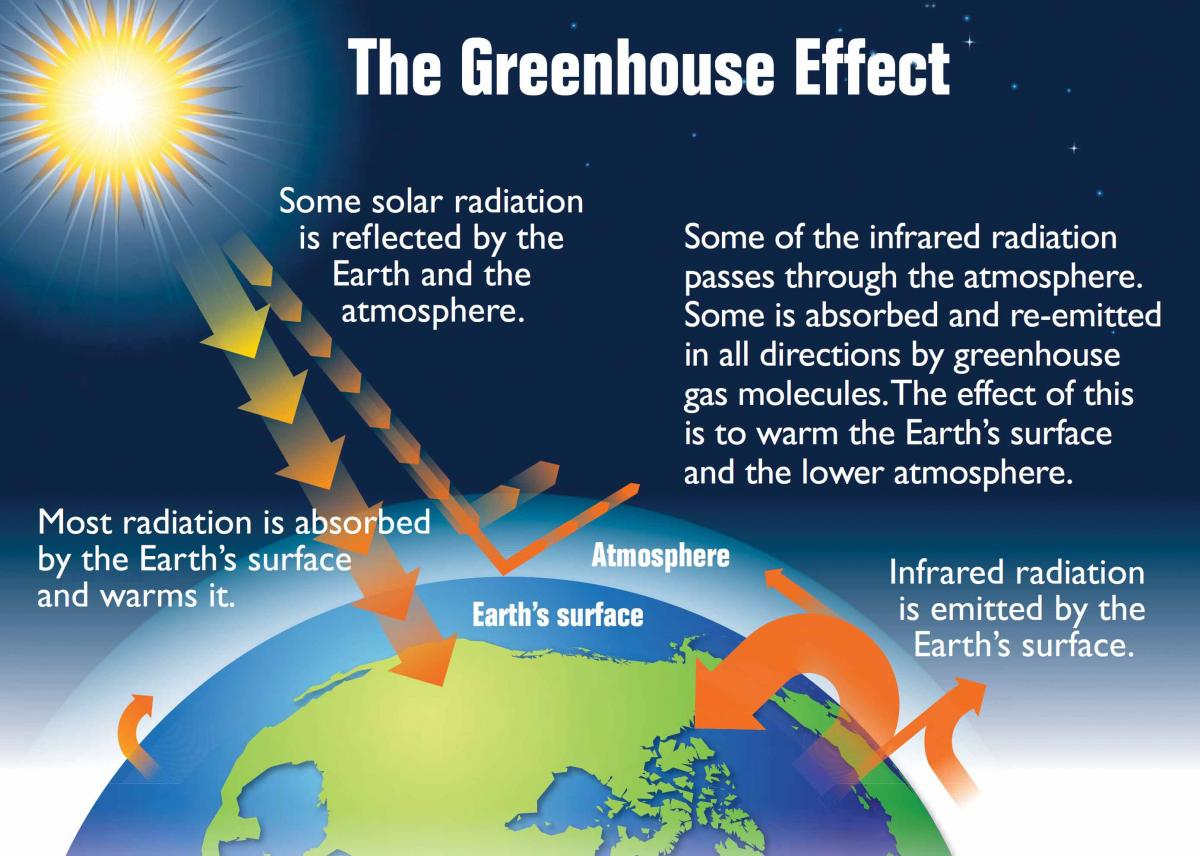
\includegraphics{./assets/greenhouse-effect.jpg}
\end{tcolorbox}

\hypertarget{climate-change-assessments}{%
\chapter{Climate Change Assessments}\label{climate-change-assessments}}

A growing awareness of our changing global climate since the 1950s has
led to a substantial body of research. For example, the National Academy
of Sciences (NAS 2011) report, American's Climate Choices, stated:

\begin{quote}
Climate change is occurring, is very likely caused primarily by human
activities, and poses significant risks to humans and the environment.
These risks indicate a pressing need for substantial action to limit the
magnitude of climate change and to prepare for adapting to its impacts.
\end{quote}

In 1990, the United Nations tasked the Intergovernmental Panel on
Climate Change (IPCC, see sidebar) with assessing existing research on
climate change. Since then, five IPCC assessments have increased our
scientific understanding of, and certainty about, global climate change.
As described later in this chapter, the assessments have incorporated
increasingly sophisticated models and analyses that consider both
natural and human contributions to changes in our climate system.

In its most recent Fifth Assessment Report, the IPCC raised the
likelihood of changes in several global climate events to ``virtually
certain'' (i.e., 99-100\% likelihood). Examples of these events include:
more frequent hot days, less frequent cold days, reductions in
permafrost, and sea-level rise (IPCC 2014).

\begin{tcolorbox}[standard jigsaw,colbacktitle=quarto-callout-note-color!10!white, bottomtitle=1mm, toptitle=1mm, rightrule=.15mm, leftrule=.75mm, titlerule=0mm, title={What is the IPCC}, arc=.35mm, bottomrule=.15mm, colframe=quarto-callout-note-color-frame, opacityback=0, opacitybacktitle=0.6, colback=white, left=2mm, toprule=.15mm, coltitle=black]
The Intergovernmental Panel on Climate Change is the leading
international body for the assessment of climate change. It was
established in 1988 by the United Nations Environment Programme and the
World Meteorological Organization, and subsequently endorsed by the
United Nations General Assembly. The goal of the IPCC is to provide the
world with a clear scientific view on the current state of knowledge in
climate change and its potential environmental and socioeconomic
impacts.


\includegraphics{./assets/ipcc.jpg}
\end{tcolorbox}

Recently, the third National Climate Assessment, produced in
collaboration with the US Global Change Research Program, provided
further insight into the anticipated climate changes for the
conterminous US. The National Climate Assessment (NCA 2014) states:

\begin{quote}
Evidence for changes in Earth's climate can be found from the top of the
atmosphere to the depths of the oceans. Researchers from around the
world have compiled this evidence using satellites, weather balloons,
thermometers at surface stations, and many other types of observing
systems that monitor the Earth's weather and climate. The sum total of
this evidence tells an unambiguous story: the planet is warming.
\end{quote}

\hypertarget{alaskas-observed-climate}{%
\chapter{Alaska's Observed Climate}\label{alaskas-observed-climate}}

To put future Montana climate change in perspective, we must first
understand Montana's baseline (i.e., historical) conditions. In this
section, we describe our state's unique geography and topography, as
well as current climatology and the historical climate trends that have
led us to the present day.

Alaska

\hypertarget{references}{%
\chapter*{References}\label{references}}
\addcontentsline{toc}{chapter}{References}

\hypertarget{refs}{}
\begin{CSLReferences}{0}{0}
\end{CSLReferences}


\end{document}
